\section{Comparing synchronisation linearisation and standard linearisation}
\label{sec:relating}

In this section we describe the relationship between synchronisation
linearisation and standard linearisation.

It is clear that synchronisation linearisation is equivalent to standard
linearisation in the (rather trivial) case that no operations actually
synchronise, so each operation of the synchronisation specification object
corresponds to a single operation of the concurrent object.  Put another way:
standard linearisation is an instance of synchronisation linearisation with
just unary synchronisations.

However, linearisability and synchronisation linearisability are not
equivalent in general: we show that, given a synchronisation linearisability
specification object |SyncSpec|, it is not always possible to find a
linearisability specification |Spec| such that for every concurrent
history~$h$,\, $h$ is synchronisation linearisable with respect to |SyncSpec|
if and only if $h$ is linearisable with respect to |Spec|.

For example, consider the example of a synchronous channel from
Section~\ref{sec:spec}, where synchronisation linearisation is captured by
|SyncChanSpec|.  Assume (for a contradiction) that the same property can be
captured by linearisation with respect to linearisability
specification~|Spec|.  Consider the history
\begin{eqnarray*}
h & = & \seq{ 
  \call.\send^1(3),\, \call.\receive^2(),\, 
  \return.\send^1\::(),\, \return.\receive^2()\::3 }.
\end{eqnarray*}
%
This is synchronisation linearisable with respect to |SyncChanSpec|.  By the
assumption, it must also be linearisable with respect to~|Spec|; so there must
be a legal history~$h_s$ of~|Spec| such that $h_s$ is a linearisation of~$h$.
Without loss of generality, suppose the |send| in~$h_s$ occurs before
the~|receive|, i.e.
\begin{eqnarray*}
h_s & = & \seq{ \send^1(3)\::(),\, \receive^2()\::3 }.
\end{eqnarray*}
%
But the history
%
\begin{eqnarray*}
h' & = & \seq{ 
  \call.\send^1(3),\, \return.\send^1\::(),\, 
  \call.\receive^2(),\, \return.\receive^2()\::3 }
\end{eqnarray*}
%
is also linearised by~$h_s$, so $h'$ is linearisable with respect to~|Spec|.
But then the assumption would imply that $h'$ is synchronisation linearisable
with respect to~|SyncChanSpec|.  This is clearly false, because the operations
do not overlap.  Hence no such linearisability specification~|Spec| exists.


%%%%%%%%%%%%%%%%%%%%%%%%%%%%%%%%%%%%%%%%%%%%%%%%%%%%%%%

\subsection{Two-step linearisability}

We now show that binary heterogeneous synchronisation linearisability
corresponds to a small adaptation of linearisability, where one of the
operations on the synchronisation object corresponds to \emph{two} operations
of the linearisability specification object.  We define what we mean by this,
and then prove the correspondence in the next subsection.  We generalise to
synchronisations of more than two threads, and to the homogeneous case in
Section~\ref{ssec:relating-variations}.  In the definitions below, we describe
just the differences from standard linearisation, to avoid repetition.

Given a synchronisation object with signature
% |op|\s1 and |op|\s2,
\begin{scala}
class SyncObj{
  def op£\s1£(x£\s1£: A£\s1£): B£\s1£
  def op£\s2£(x£\s2£: A£\s2£): B£\s2£
}
\end{scala}
we will consider a linearisability specification object with signature
%
\begin{scala}
class TwoStepLinSpec{
  def op£\s1£(x£\s1£: A£\s1£): Unit
  def £$\overline{\sm{op}}_1$£(): B£\s1£
  def op£\s2£(x£\s2£: A£\s2£): B£\s2£
}
\end{scala}
%
The idea is that the operation |op|\s1 on |SyncObj| will be linearised by the
composition of the two operations |op|\s1 and $\overline{\sm{op}}_1$ of
|TwoStepLinSpec|; but operation |op|\s2 on |SyncObj| will be linearised by
just the operation |op|\s2 of |TwoStepLinSpec|, as before.  We call such an
object a \emph{two-step linearisability specification object}.

We define a legal history~$h_s$ of such a two-step specification object much
as in Section~\ref{sec:specification-linearisability}, with the addition that
for each event $\overline{\sm{op}}_1^i()\::y$ in~$h_s$, we require that there
is an earlier event |op|$_1^i(x)\::()$ in~$h_s$ with the same invocation
identity; other than in this regard, invocation identities are not repeated
in~$h_s$.

Let $h$ be a complete concurrent history of a synchronisation object, and let
$h_s$ be a legal history of a two-step specification object corresponding to
the same invocations in the following sense:
%
\begin{itemize}
\item For every $\call.\sm{op}_1^i(x)$ and $\return.\sm{op}_1^i\::y$ in $h$,\,
  $h_s$~contains $\sm{op}_1^i(x)\::()$ and $\overline{\sm{op}}_1^i()\::y$; and
  vice versa;

\item For every $\call.\sm{op}_2^i(x)$ and $\return.\sm{op}_2^i\::y$ in $h$,\,
  $h_s$~contains $\sm{op}_2^i(x)\::y$; and vice versa.
\end{itemize}
%
We say that $h_s$ is a \emph{two-step linearisation} of~$h$ if there is some
way of interleaving the two histories such that
%
\begin{itemize}
\item Each $\sm{op}_1^i(x)\::()$ and $\overline{\sm{op}}_1^i()\::y$ occur
  between $\call.\sm{op}_1^i(x)$ and $\return.\sm{op}_1^i\::y$, in that
  order; 

\item Each $\sm{op}_2^i(x)\::y$ occurs between $\call.\sm{op}_2^i(x)$ and
  $\return.\sm{op}_2^i\::y$.
\end{itemize}

For example, consider a synchronous channel, with |send| corresponding
to~$\op_1$, and |receive| corresponding to~$\op_2$.  Then the following would
be an interleaving of a history of the channel and a two-step linearisation.
\[
\seq{\begin{align} 
 \call.\sm{send}^1(3),\; \sm{send}^1(3)\::(),\; 
 \call.\sm{receive}^2(),\; \sm{receive}^2()\::3,\; \\
 \overline{\sm{send}}^1()\::(),\; \return.\sm{send}^1\::(), \;
 \return.\sm{receive}^2\::3 }.
\end{align}
\]
%
%\framebox{timeline to illustrate}
This is represented by the following timeline, where the horizontal lines and
the labels above represent the interval between the $\call$ and $\return$
events of the synchronisation object, and the ``$\cross$''s and the labels
below represent the corresponding operations of the specification object.
%  
\begin{center}
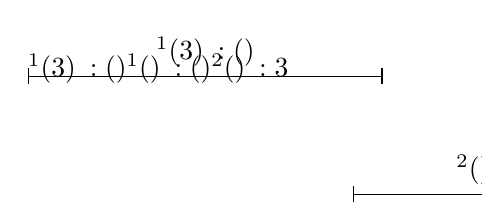
\begin{tikzpicture}[xscale = 0.9]
\draw[|-|] (0,0) -- node[above] {$\send^1(3)\::()$} (5,0);
\crossAt(1,0){$\send^1(3)\::()$}
\crossAt(4,0){$\overline{\send}^1()\::()$}
%\draw (1, 0) \X; \draw(4,0) \X;
\draw[|-|] (2,-1.5) -- node[above] {$\receive^2()\::3$} (6,-1.5);
\crossAt(3,-1.5){$\receive^2()\::3$}
%\draw(3,-1.5) \X;
\end{tikzpicture}
\end{center}

The definition of two-step linearisability of a synchronistion object then
follows from this definition of two-step linearisation of complete histories,
precisely as in Section~\ref{sec:specification-linearisability}.


%%%%%%%%%%%%%%%%%%%%%%%%%%%%%%%%%%%%%%%%%%%%%%%%%%%%%%%

\subsection{Proving the relationship}
\label{sec:twoStepLinSpec}

We now prove the relationship between synchronisation linearisation and
two-step linearisation.
%
Consider a synchonisation specification object |Sync|\-|Spec|.  We build a
corresponding two-step linearisation specification object |Two|\-|StepLinSpec|
such that synchronisation linearisation with respect to |Sync|\-|Spec| is
equivalent to two-step linearisation with respect to
|Two|\-|Step|\-|Lin|\-|Spec|.  The definition we choose is not the simplest
possible, but it is convenient for the testing framework we use in
Section~\ref{sec:testing-hacking}.

The definition of |TwoStepLinSpec| is below.  We assume that each thread has
an identity in some range $\range 0 {\sm{NumThreads}}$.  For simplicity, we
arrange for this identity to be included in the $\call$ events for
operations~|op|\s1 and $\overline{\sm{op}}_1$.
%%  (Alternatively, we
%% could implement thread identities internally to the object, for example using
%% the technique from~\cite[Appendix~A.2.4]{herlihy-shavit}.)

The object |TwoStepLinSpec| requires that corresponding invocations of~|op|\s1
and~|op|\s2 are linearised consecutively: it does this by encoding the
automaton on the right.  However, it allows the corresponding
$\overline{\sm{op}}_1$ to be linearised later (but before the next operation
invocation by the same thread).  It uses an array |returns|, indexed by thread
identities, to record the value that should be returned by an
$\overline{\sm{op}}_1$ invocation by each thread.  Each invocation of $\op_2$
calls |SyncSpec.sync| to obtain the values that should be returned for
synchronisation linearisation; it writes the value for the corresponding
$\overline\op_1$ into |returns|.
%
\begin{trivlist}
\item[]
\begin{minipage}{92mm}
\begin{scala}
type ThreadID = Int              // Thread identifiers
val NumThreads: Int = ...       // Number of threads
trait State
case object Zero extends State
case class One(t: ThreadID, x£\s1£: A£\s1£) extends State
\end{scala}
\end{minipage}
%%%%%
\hfill 
%
\begin{minipage}{39mm}
\begin{tikzpicture}[>= angle 60, xscale = 0.9, yscale = 0.44]
\draw (0,0) node[draw] (zero) {$\sm{Zero}$};
\draw[->] (zero) ++ (-1.5, 0) -- (zero);
%\draw (zero)++(0.2,0) node (zz) {};
\loopAbove(zero){$\begin{array}{c}
  \overline\op_1(\sm t) \\ {[\sm{returns(t)} \ne \sm{None}]}
  \end{array}$}
%% \draw[->] (zero) .. controls ++(1.2,+1.0) and ++(1.2,-1.0) .. 
%%   node[right] {$\overline\op_1(\sm t)$} (zero);
%
\draw (0,-4) node[draw] (one) {$\sm{One}(\sm t, \sm{x}_1)$};
\draw[->] (zero) .. controls ++(0.3,-2) .. 
  node[right] {$\sm{op}_1(\sm t, \sm{x}_1)$} (one); 
%
\draw[->] (one) .. controls ++(-0.3,2) .. 
  node[left] {$\sm{op}_2(\sm x_2)$} (zero);
\end{tikzpicture}%
\end{minipage}%
%%%%%
\begin{scala}
object TwoStepLinSpec{
  private var state: State = Zero
  private val returns = new Array[Option[B£\s1£]](NumThreads)
  for(t <- 0 until NumThreads) returns(t) = None
  def op£\s1£(t: ThreadID, x£\s1£: A£\s1£): Unit = {
    require(state == Zero && returns(t) == None); state = One(t, x£\s1£); ()
  }
  def op£\s2£(x£\s2£: A£\s2£): B£\s2£ = {
    require(state.isInstanceOf[One]); val One(t, x£\s1£) = state
    val (y£\s1£, y£\s2£) = SyncSpec.sync(x£\s1£, x£\s2£); returns(t) = Some(y£\s1£); state = Zero; y£\s2£
  }
  def £$\overline{\sm{op}}_1$£(t: ThreadID): B£\s1£ = {
    require(state == Zero && returns(t).isInstanceOf[Some[B£\s1£]])
    val Some(y£\s1£) = returns(t); returns(t) = None; y£\s1£
  }
}
\end{scala}
\end{trivlist}

%%%%%

%% \framebox{Do we want to talk about \emph{complete} histories of
%%   TwoStepDelayedLinSpec?} -- containing all three events of a set

The following lemma identifies important properties of
|Two|\-|Step|\-|LinSpec|.  It follows immediately from the
definition.
%
\begin{lemma}
\label{lem:TwoStepLinSpec-histories}
Within any legal history of |TwoStepLinSpec|, events $\op_1$ and
$\op_2$ alternate.  Let $\op_1^{i_1}(t,x_1) \:: ()$ and $\op_2^{i_2}(x_2) \::
y_2$ be a consecutive pair of such events.  Then |op|\s2 makes a call
$\sm{SyncSpec.sync}(x_1, x_2)$ obtaining result $(y_1,y_2)$.  The next event
for thread~$t$ (if any) will be $\overline\op_1^{i_1}(t) \:: y_1$; and this
will be later in the history than $\op_2^{i_2}(x_2) \:: y_2$.  Further, the
corresponding history of events $\sm{sync}^{i_1,i_2}(x_1,x_2) \:: (y_1,y_2)$
is a legal history of |SyncSpec|.

Conversely, each history with events ordered in this way will be a legal
history of |TwoStepLinSpec| if  the corresponding history
of events $\sm{sync}^{i_1,i_2}(x_1,x_2) \:: (y_1,y_2)$ is a legal history of
|SyncSpec|.
\end{lemma}

%%%%%

The following proposition reduces synchronisation linearisability to two-step
linearisability.
%
\begin{prop}
\label{prop:two-step-lin}
Let |SyncObj| be a binary heterogeneous synchronisation object, |SyncSpec| a
corresponding synchronisation specification object, and let |TwoStepLinSpec|
be built from |SyncSpec| as above.  Then each history~$h$ of |SyncObj| is
two-step linearisable with respect to |Two|\-|Step|\-|LinSpec| if and only if
it is synchronisation linearisable with respect to |SyncSpec|.  And hence
|SyncObj| is two-step linearisable with respect to |Two|\-|Step|\-|LinSpec| if
and only if it is synchronisation linearisable with respect to |SyncSpec|.
\end{prop}
%%%%%%
\begin{proof}
\textbf{($\implies$).}\quad
%
Let $h$ be a concurrent history of |SyncObj|.  By assumption, there is an
extension $h'$ of~$h$, and a legal history~$h_s$ of |TwoStepLinSpec| such that
$h_s$ is a  two-step linearisation of $h'' = complete(h')$.
%
Build a history~$h_s'$ of |SyncSpec| by replacing each consecutive pair
$\sm{op}_1^{i_1}(x_1) \:: ()$,\, $\sm{op}_2^{i_2}(x_2) \:: y_2$ in~$h_s$ by
the event $\sm{sync}^{i_1,i_2}(x_1,x_2) \:: (y_1,y_2)$, where $y_1$ is the
value returned by the corresponding~$\overline{\sm{op}}_1^{i_1}()$.
%
This is illustrated by the example timeline below, where $h''$ is represented
by the horizontal lines and the labels above; $h_s$ is represented by the
``$\cross$''s and the labels below; and $h_s'$ is represented by the
``$\bullet$'' and the label below.
%
\begin{center}
\begin{tikzpicture}[xscale = 0.9]
\draw[|-|] (0,0) -- node[above] {$\send^1(3)\::()$} (7,0);
\crossAt(1,0){$\send^1(3):()$}
%\draw (1, 0) \X; \draw (1,-0.4) node{$\sm{send}^1(3):()$}; 
\crossAt(6,0){$\overline{\send^1}():()$}
%\draw(6,0) \X; \draw(6,-0.4) node{$\overline{\sm{send}^1}():()$};
%
\draw[|-|] (2,-1.5) -- node[above] {$\receive^2()\::3$} (5,-1.5);
\crossAt(3,-1.5){$\receive^2()\::3$};
%\draw(3,-1.5) \X; \draw(3,-1.9) node{$\sm{receive}^2()\::3$};
%
\draw(3,-2.5) node{$\bullet$}; 
\draw(3,-2.9) node{$\sm{sync}^{1,2}(3,()): ((),3)$};
\end{tikzpicture}
\end{center}

The history~$h_s'$ is legal for |SyncSpec| by
Lemma~\ref{lem:TwoStepLinSpec-histories}.
%
It is possible to interleave $h''$ and~$h_s'$ by placing each event
$\sm{sync}^{i_1,i_2}(x_1,x_2) \:: (y_1,y_2)$ in the same place as the
corresponding event $\sm{op}_2^{i_2}(x_2) \:: y_2$ in the interleaving
of~$h''$ and~$h_s$; by construction, this is between
$\call.\sm{op}_1^{i_1}(x_1)$ and~$\return.\sm{op}_1^{i_1} \:: y_1$, and
between $\call.\sm{op}_2^{i_2}(x_2)$ and~$\return.\sm{op}_2^{i_2} \:: y_2$.
%
Hence $h_s$ is a synchronisation linearisation of~$h''$; and so $h$ is
synchronisation-linearisable.

%%%%%

\textbf{($\Leftarrow$).}\quad
%
Let $h$ be a complete history of |SyncObj|.  By assumption, there is an
extension $h'$ of~$h$, and a legal history~$h_s$ of |SyncSpec| such that $h_s$
is a synchronisation linearisation of $h'' = complete(h')$.
%
Build a history~$h_s'$ of |TwoStepLinSpec| by replacing each event
$\sm{sync}^{i_1,i_2}(x_1,x_2) \:: (y_1,y_2)$ in~$h_s$ by the three consecutive
events $\sm{op}_1^{i_1}(x_1) \:: ()$,\, $\sm{op}_2^{i_2}(x_2) \:: y_2$,\,
$\overline{\sm{op}}_1^{i_1}() \:: y_1$.

The history~$h_s'$ is legal for |TwoStepLinSpec| by
Lemma~\ref{lem:TwoStepLinSpec-histories}.
%
It is possible to interleave $h''$ and~$h_s'$ by placing each triple
$\sm{op}_1^{i_1}(x_1) \:: ()$,\, $\sm{op}_2^{i_2}(x_2) \:: y_2$,\,
$\overline{\sm{op}}_1^{i_1}() \:: y_1$ in the same place as the corresponding
event $\sm{sync}^{i_1,i_2}(x_1,x_2) \:: (y_1,y_2)$ in the interleaving
of~$h''$ and~$h_s$; by construction, each $\sm{op}_1^{i_1}(x_1) \:: ()$ and
$\overline{\sm{op}}_1^{i_1}() \:: y_1$ are between
$\call.\sm{op}_1^{i_1}(x_1)$ and~$\return.\sm{op}_1^{i_1} \:: y_1$; and each
$\sm{op}_2^{i_2}(x_2) \:: y_2$ is between $\call.\sm{op}_2^{i_2}(x_2)$
and~$\return.\sm{op}_2^{i_2} \:: y_2$.
%
Hence $h_s$ is a two-step linearisation of $h''$; and so $h$ is
two-step-linearisable.
\end{proof}

The two-step linearisation specification object can often be significantly
simplified from the template definition above.  Here is such a specification
object for a synchronous channel.
%
\begin{scala}
object SyncChanTwoStepLinSpec{
  private var state = 0           // Takes values 0, 1, cyclically 
  private var threadID = -1    // Current sender's thread ID when state = 1
  private var value: A = _      // The current value being sent when state = One
  private val canReturn =       // which senders can return?
    new Array[Boolean](NumThreads) 
  def send(t: ThreadID, x: A): Unit = { 
    require(state == 0 && !canReturn(t)); value = x; threadID = t; state = 1 }
  def receive(u: Unit): A = { 
    require(state == 1); canReturn(threadID) = true; state = 0; value }
  def £$\overline{\send}$£(t: ThreadID): Unit = { 
    require(state == 0 && canReturn(t)); canReturn(t) = false }
}
\end{scala}
